\documentclass[a4paper,10pt]{article}
\usepackage[T1]{fontenc}
\usepackage[utf8]{inputenc}
\usepackage{lmodern}
\usepackage{indentfirst}
\usepackage{graphicx}
\usepackage{listings}
\usepackage{hyperref}

\title{Automated Groceries Storage: Fridge or Non-Fridge decision}

\begin{document}

\maketitle 

\section{Domain Background}

There are huge advancements in Robotics that helps in Supermarkets orders fulfillment, checking, and maintaining stock \cite{supermarketrobots} . However, the products are bought for millions of people and took it into their home, and they don't have robots to help you with the everyday chores. \\

At home, the groceries storage is done item by item by a human where one of the most important decision is to determine the proper storage of each product according to the places in the home and the conservation requirements of the product.\\

This task consumes time. My particular interest is to build technology that helps to carry out each of the household tasks. \\

Some initiatives in Computer Vision and Deep Learning for detecting products where propopsed. See "The Freiburg Groceries DataSet" Philipp Jund at el. \cite{freiburgpaper}  

\section{Problem Statement}

At home, the storage of grocery products could be simplified to \textbf{this item should go in the fridge or not}. To preserve the conservation chain, some products need to be stored in the refrigerator.\\

The idea is to build a system that can detect if an item should be stored in the fridge or not, using Deep Learning. \\

So, the problem is simplified to a bi-categorical classification: Fridge or not Fridge. \\


\section{Data sets and Inputs}

There are few grocery products datasets over the web ready for Deep Learning. One example is "The Freiburg Groceries Dataset" consists of 5000 256x256 RGB images of 25 food classes. Figure 1.2 shows some sample images. \\

\begin{figure}
  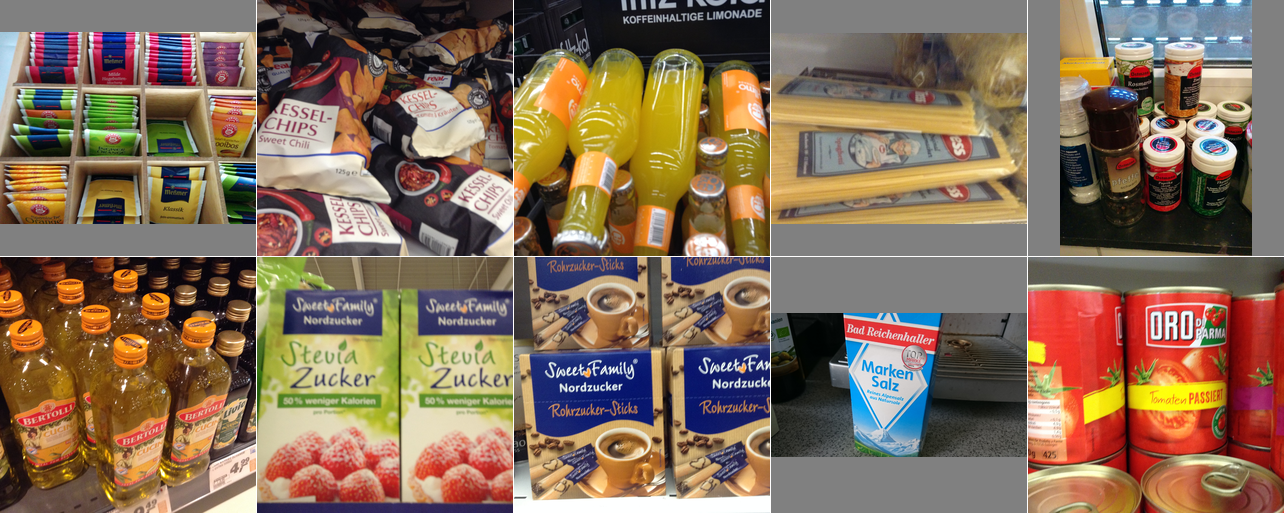
\includegraphics[width=\linewidth]{examples.png}
  \caption{Freiburg Groceries Dataset}
  \label{fig:boat1}
\end{figure}


But the images includes several products. \\

The "Precios Cuidados" products dataset is going to be used. "Precios Claros" is an argentinian initiative that collects prices of different supermarkets in order to protect the rights of the buyers. \\

The product's images could be downloaded using a public API. \\

\begin{figure}
  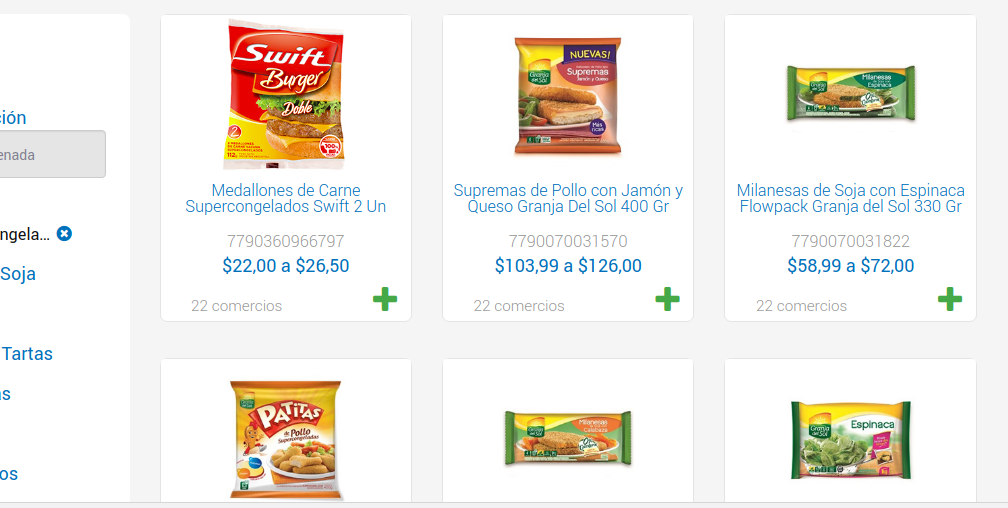
\includegraphics[width=\linewidth]{products.png}
  \caption{Precios Claros Dataset Example}
  \label{fig:boat1}
\end{figure}

About the database preparation, the "Precios Cuidados" dataset is labeled by category. A "fridge or no fridge" labeled will be required. The idea is to manually tags the products. \\ 

The dataset includes around 4685 images and it only includes one version of each product. It includes 711 fridge products and 3975 non-fridge labeled products. \\

Data Augmentation will be required to increase the samples different views and help to reach higher accuracies. More than 10.000 in total in the dataset will be used. The separation will be 75\% train, 15\% validate, and 10\% test. And it will mantain the original proporsion of frige/non-fridge products in each subset.\\

\section{Solution statement}

The objective of the present work is to analyze and provide a Convolutional Neural Network that could serve as a starting point of the robot software.\\

This CNN should detect using a product image if the item were stored in the refrigerator or not. The approach will be to select the best CNN network built from scratch.\\

\section{Benchmark Model}

This is a novel project. No previous work on fridge/non-fridge products detection is available online. To benchmark, the network solution, a model with transfer learning VGG16\cite{vgg16}. \\

VGG16\cite{vgg16} pre-trained model was generated over ImageNet dataset during weeks. As we have seen in the Dog Breed project, their performance in other domains is great. \\

\section{Evaluation Metrics}

At training time, the accuracy will be used to measure the success of the network. Also, the loss and validation loss progress will be checked to provided an accurate model without underfitting or overfitting conditions.\\

The final score will be given by the \textbf{F1-score} over the test dataset.

\section{Project Design}

The project will need to accomplish the following points:
\begin{itemize}
  \item Dataset preparation
  \item Algorithms and Techniques description
  \item Benchmark Model (transfer learning model)
  \item CNN from scratch 
  \item Model Evaluation
  \item Conclusions
\end{itemize}

Each item will be achieved in order.


\subsection{Dataset preparation}

Pre-process steps: 
\begin{itemize}
  \item Includes to download and resize the "Precios Cuidados" images.
  \item Apply data augmentation 
  \item Separate the data in train-validation-test
  \item Complete Data Exploration and Exploratory Visualization report sections.
\end{itemize}

\subsection{Algorithms and Techniques description}

This section I will include a description of transfer learning and Convolutional Neural Networks. 

\subsection{Benchmark Model}

I will extract VGG16 bottleneck features and use the simple model from Dog Breed Classifier project applied over the dataset

\begin{lstlisting}
model = Sequential()
model.add(GlobalAveragePooling2D(input_shape=bottleneck_features.shape[1:]))
model.add(Dense(2, activation='softmax'))
\end{lstlisting}

The training will be using rmsprop optimizer and categorical\_crossentropy loss (bi-categorical) 

After that, the obtained accuracy is going to serve as benchmark. Next step, will be to complete Benchmark model report section.

\subsection{CNN Model}

\begin{itemize}
\item Implement a Neural Network from scratch
\item Select loss function and optimizer. Different optimizers could be tried: Adamax, Adam, RMSProp
\item Adjust the hyperparameters to increase accuracy
\item Complete Implement and Refinement
\end{itemize}

About the CNN, the idea is to use Conv2D layers with Dropout (to prevent overfitting) and BatchNormalization to normalize the inputs in some layers. \\

To perform the hyperparmeter tunning, the idea is to use grid search. \\ 
 
\subsection{Model Evaluation}

\begin{itemize}
\item Compare the best CNN Model with the Benchmark Model
\item Use the CNN for prediting in 10 sample images at least
\item Complete Model Evaluation and Validation
\end{itemize}

\subsection{Conclusions}

Complete the Justification and Conclusion section of the project report. 

%https://www.fastcodesign.com/90150368/this-online-supermarkets-robots-put-your-order-together-in-minutes
%https://www.technologyreview.com/s/603229/the-robotic-grocery-store-of-the-future-is-here/
%http://aisdatasets.informatik.uni-freiburg.de/freiburg_groceries_dataset/
%https://arxiv.org/pdf/1611.05799.pdf
%https://www.preciosclaros.gob.ar/#!/buscar-productos

\begin{thebibliography}{9}
\bibitem{supermarketrobots} 
\textit{Super Market Robots}. 
\url{https://www.fastcodesign.com/90150368/this-online-supermarkets-robots-put-your-order-together-in-minutes} 

\bibitem{preciosclaros} 
\textit{Precios Claros} 
\url{https://www.preciosclaros.gob.ar/\#!/buscar-productos}
 
\bibitem{freiburg} 
\textit{Freiburg groceries dataset} 
\url{http://aisdatasets.informatik.uni-freiburg.de/freiburg\_groceries\_dataset/}

\bibitem{freiburgpaper} 
\textit{Freiburg groceries paper}
\url{https://arxiv.org/abs/1611.05799} 

\bibitem{vgg16}
\textit{VGG16 Paper}
\url{https://arxiv.org/abs/1409.1556}


\end{thebibliography}
 

\end{document}
